\section{实验结果}
通过正则表达式\verb|(\d+)\/(\d+)℃|,可以从selenium获取到的字符串中提取出每日的最高温度和最低温度。
9月份上海市每日的最高温度和最低温度的变化情况如图\ref{maxmin}所示。
\begin{figure}[!htbp]
    \centering
    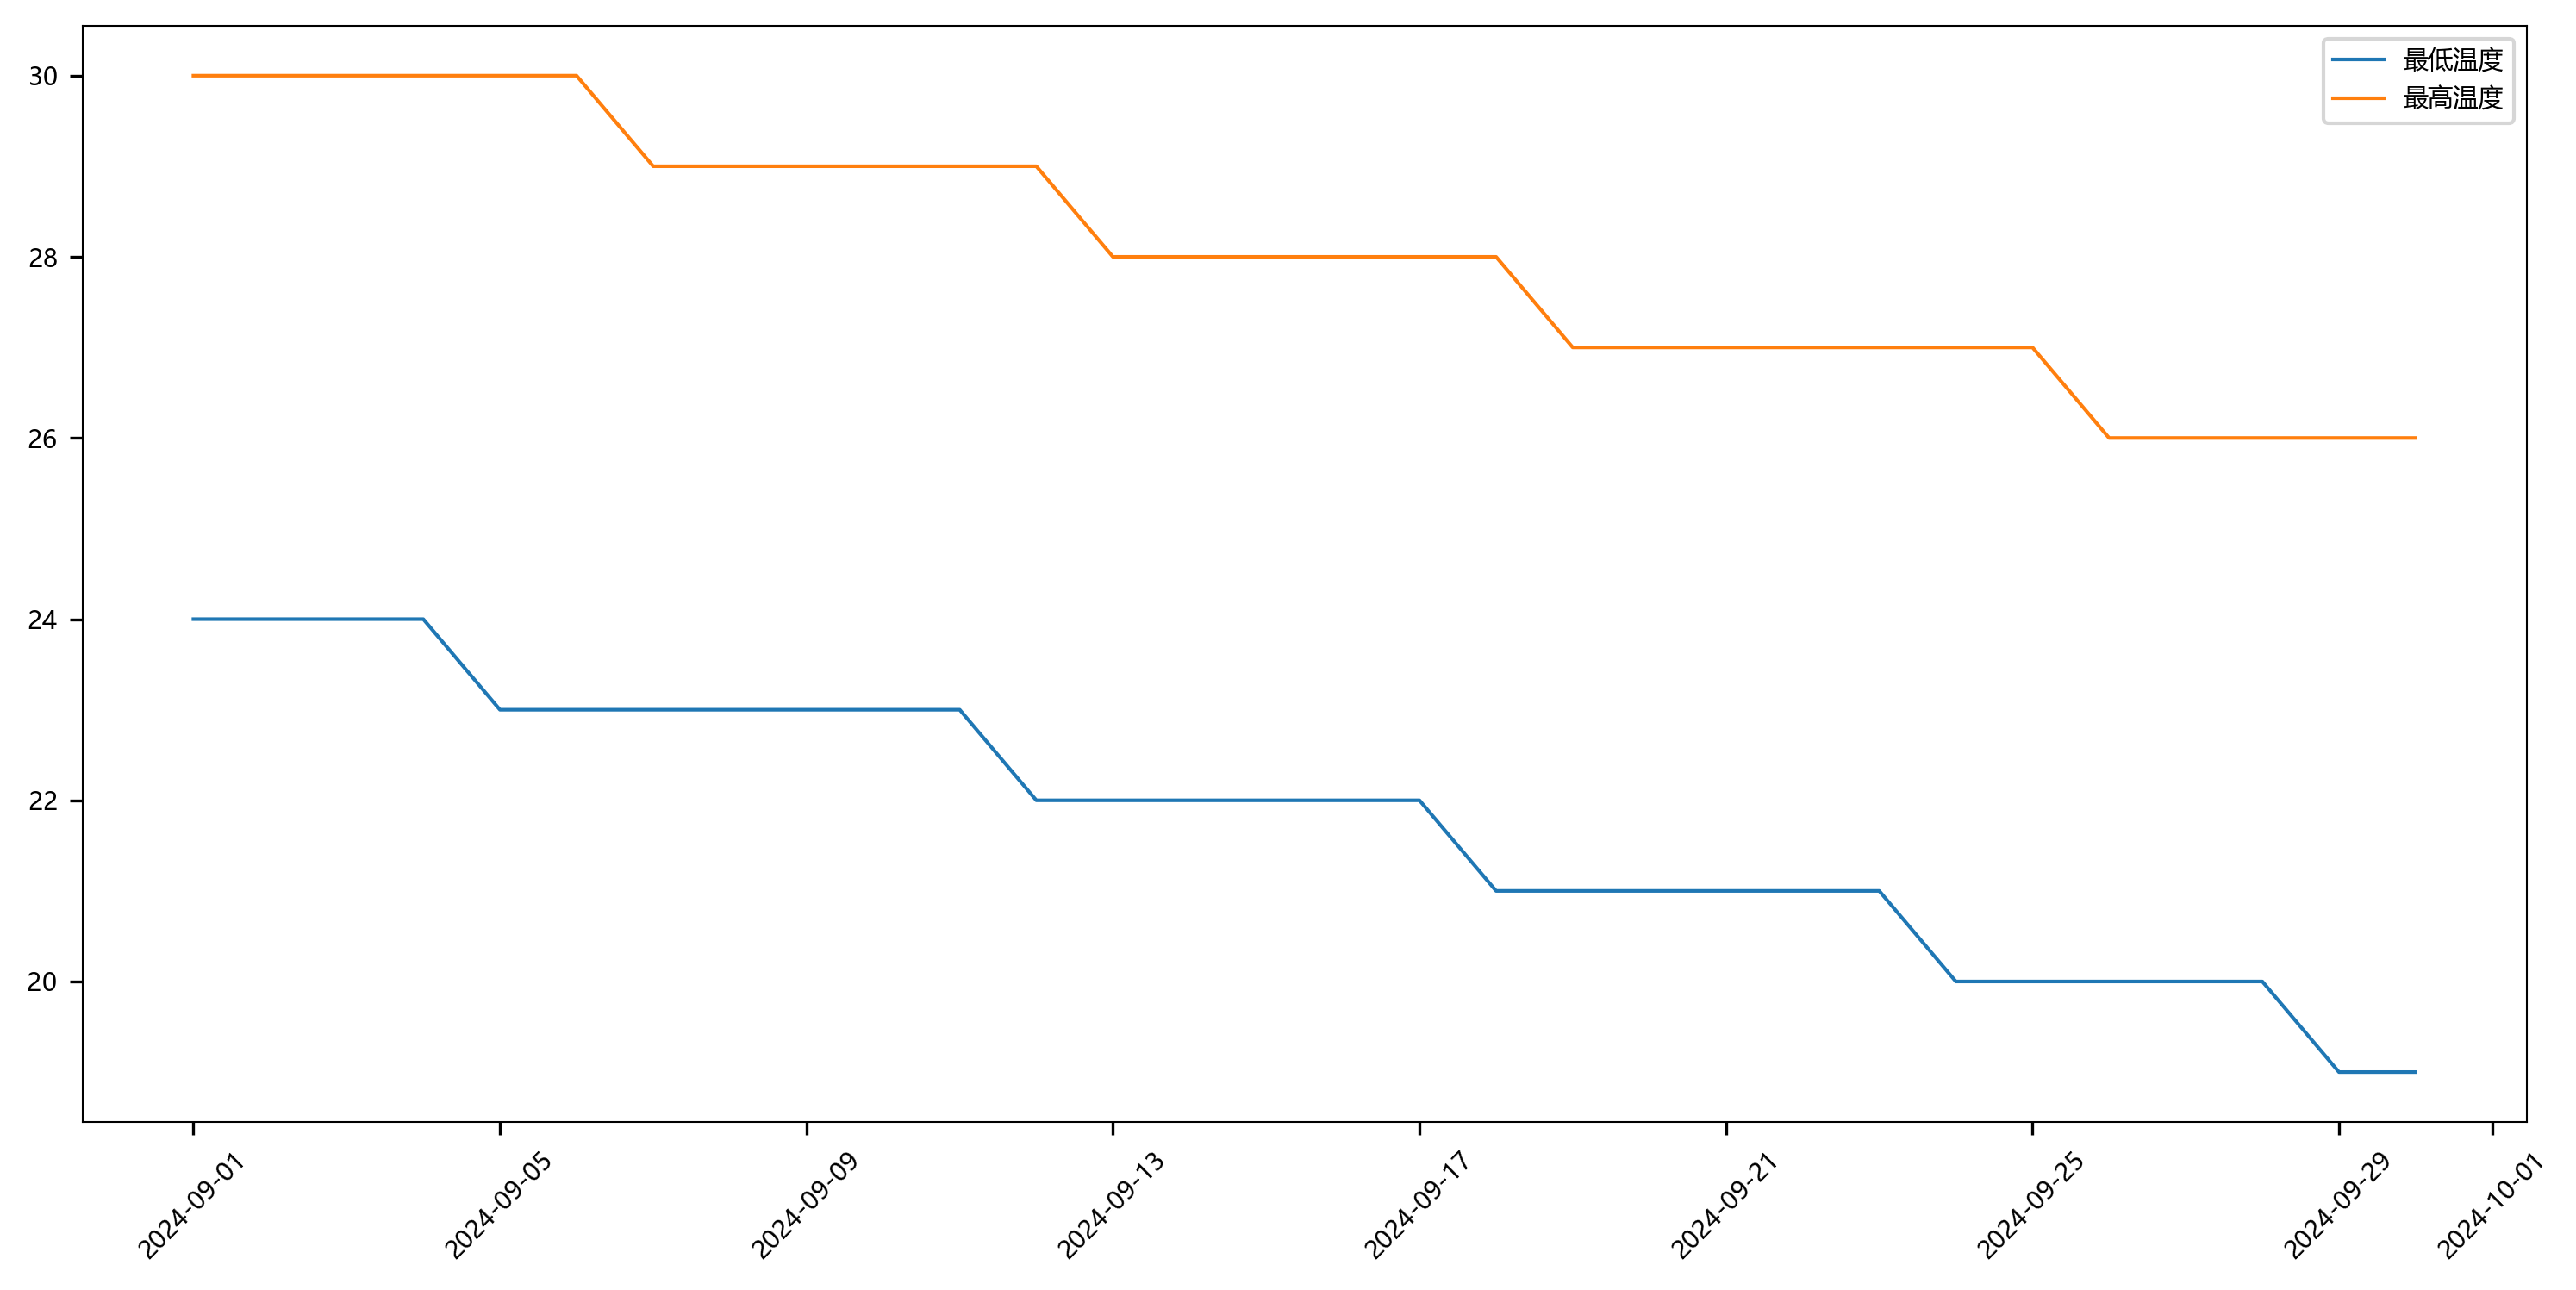
\includegraphics[width=\textwidth]{figures/max_min.png}
    \caption{9月份上海市每日的最高温度和最低温度}\label{maxmin}
\end{figure}

通过正则表达式\verb|\"n\"\:\"(.+?)\",\"x\"\:\"(.+?)\",\"y\"\:\"(.+?)\"|,可以从city的请求回复报文体
中提取出所有的城市及其经纬度,然后将它们作为载荷放入api和sk的请求报文头中,并从回复报文体中提取出城市名称信息以及气温信息,存储至SQLite数据库中,
期间利用日志记录异常的返回值。

如图\ref{csv}所示,本次实验中,我共收集了3217条数据,其中共2399个城市的天气信息,包含风力、风向、温度、天气、湿度。

\begin{figure}[!htbp]
    \centering
    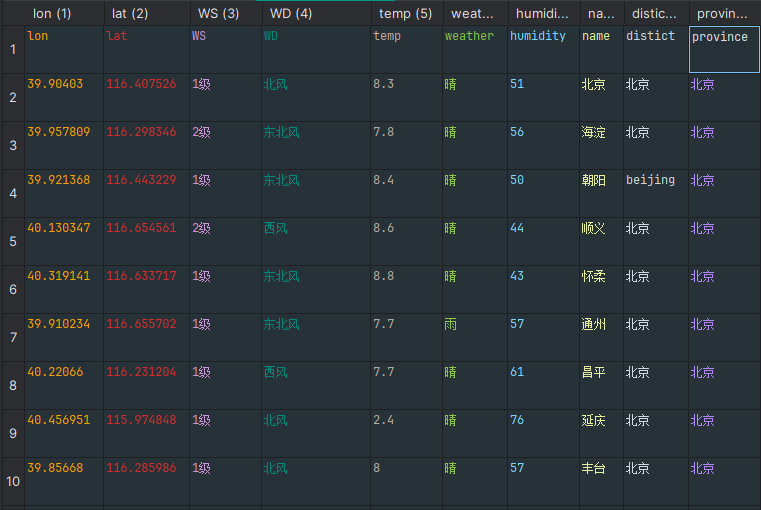
\includegraphics[width=\textwidth]{figures/csv.png}
    \caption{各城市的天气信息}\label{csv}
\end{figure}
